\documentclass{article}
\usepackage{fancyhdr}
\usepackage{lipsum}  
\usepackage{listings} 
\usepackage{xcolor}   
\usepackage{amsmath}
\usepackage{enumitem}
\usepackage{graphicx}
\usepackage{caption}
\usepackage{verbatim}

% Define macros for title and author
\newcommand{\thetitle}{STAT 641 \\ Homework 6}
\newcommand{\theauthor}{Keegan Smith}

\title{\thetitle}
\author{\theauthor}

\pagestyle{fancy}
\fancyhf{}  % Clear all header and footer fields
\fancyhead[L]{\nouppercase{\rightmark}}
\fancyhead[C]{\thetitle}  % Title in the center
\fancyhead[R]{\theauthor}  % Your name on the right

\lstset{ %
  backgroundcolor=\color{lightgray},   % choose the background color
  basicstyle=\ttfamily\small,          % size of fonts used for the code
  keywordstyle=\color{blue},           % color for keywords
  commentstyle=\color{green},          % color for comments
  stringstyle=\color{red},             % color for strings
  numbers=left,                        % where to put the line-numbers
  numberstyle=\tiny\color{gray},       % style for line-numbers
  stepnumber=1,                        % the step between two line-numbers
  numbersep=5pt,                       % how far the line-numbers are from the code
  frame=single,                        % adds a frame around the code
  rulecolor=\color{black},             % frame color
  breaklines=true,                     % automatic line breaking
  breakatwhitespace=false,             % automatic breaks should only happen at whitespace
  showspaces=false,                    % don't show spaces in the code
  showstringspaces=false,              % don't show spaces in strings
  showtabs=false,                      % don't show tabs in the code
}

\begin{document}

\maketitle
\section*{Problem 1}
\begin{enumerate}
\item To create a reference plot, we must first make it such that the Weibull is a location-scale distribution. We can accomplish this (as outlined in Handout 8) by applying the transformation: \\
\[
X = \log(Y)
\]
so if $X$ follows a log-Weibull distribution, then $Y$ follows a Weibull distribution. \\
The cdf of the log weibull is: \\
\begin{align*}
P(\ln(Y) \leq x) &= P(Y \leq e^x) \\
&= 1 - e^{-(\frac{e^x}{\alpha})^\gamma} \\
&= 1 - e^{-e^{\frac{x - \theta_1}{\theta_2}}}
\end{align*}
We can then solve for the quantile function: \\
\begin{align*}
s &= 1 - e^{-e^{\frac{x - \theta_1}{\theta_2}}} \\
\ln(-s + 1) &= -e^{\frac{x - \theta_1}{\theta_2}} \\
\ln(-\ln(-s + 1)) &= \frac{x - \theta_1}{\theta_2} \\
\theta_2 \cdot \ln(-\ln(-s + 1)) + \theta_1 &= x \\
\end{align*}
Thus we have: \\
\[
Q_z(u) = \ln(-\ln(-u + 1))
\]
We can then make the reference plot with the following R code (continued from the previous R code):
\begin{verbatim}\
x <- c(0.8402, 1.0644, 1.1298, 1.4314, 1.7795, 1.9121, 2.2343, 2.3424, 2.3559, 2.3855,
2.5734, 2.5815, 2.5893, 2.7562, 2.9040, 2.9295, 3.1124, 3.5490, 3.7684, 3.7953,
3.8846, 3.9766, 4.1918, 4.3887, 4.7106, 4.8918, 4.9716, 6.5018, 7.0740, 7.2158)
y = -log(x)
y = sort(y)
n = length(y)
weib= -y
weib= sort(weib)
i= 1:n
ui= (i-.5)/n
QW= log(-log(1-ui))
plot(QW,weib,abline(lm(weib~QW)),
main="Weibull Reference Plot",cex=.75,lab=c(7,11,7),
xlab="Q=ln(-ln(1-ui))",
ylab="y=ln(W(i))")
\end{verbatim}
\begin{figure}[htbp]
    \centering
    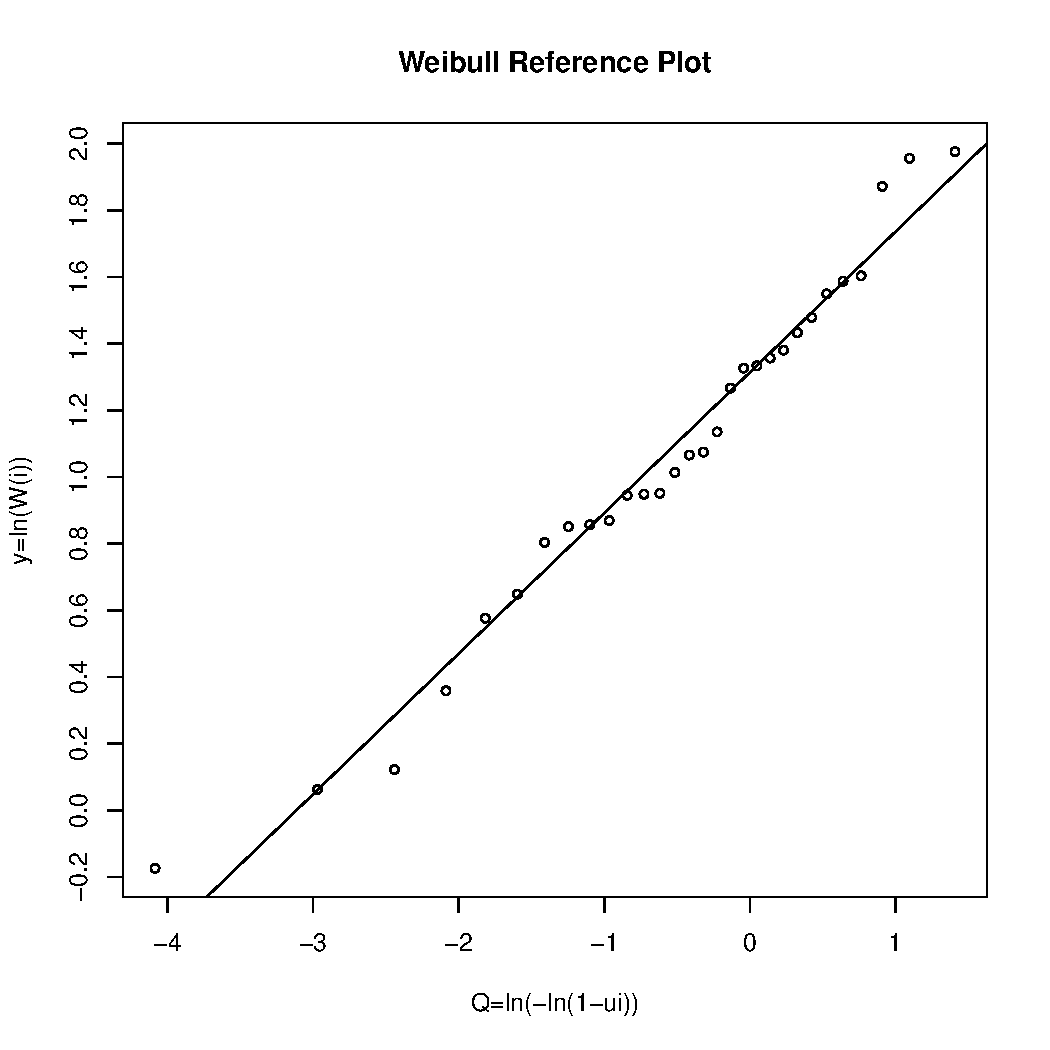
\includegraphics[width=0.8\textwidth]{Rplots.pdf}
\end{figure}
\newpage
We will also compute the Anderson-Darling GOF test in R: \\
\begin{verbatim}
library(MASS)
mle <- fitdistr(x,"weibull")
shape = mle$estimate[1]
scale = mle$estimate[2]
a = -log(scale)
b = 1/shape
z = exp(-exp(-(y-a)/b))
A1i = (2*i-1)*log(z)
A2i = (2*n+1-2*i)*log(1-z)
s1 = sum(A1i)
s2 = sum(A2i)
AD = -n-(1/n)*(s1+s2)
ADM = AD*(1+.2/sqrt(n))
AD
ADM
\end{verbatim}
This results in $A^2 = 0.3059062$. From the table in Handout 9, this corresponds with a p-value $> .25$. Combining this with the fact that the reference plot is fairly straight, I am inclined to say the Weibull distribution is a good fit for the data.
\item We can solve for the CI for the upper quantile using the following R code (adapted from handout 11): \\
\begin{verbatim}
x <- c(0.8402, 1.0644, 1.1298, 1.4314, 1.7795, 1.9121, 2.2343, 2.3424, 2.3559, 2.3855,
2.5734, 2.5815, 2.5893, 2.7562, 2.9040, 2.9295, 3.1124, 3.5490, 3.7684, 3.7953,
3.8846, 3.9766, 4.1918, 4.3887, 4.7106, 4.8918, 4.9716, 6.5018, 7.0740, 7.2158)
n=length(x)
L=.95
P=.75
s=ceiling(n*P)-1
r=floor(n*P)+1
cov=0
while(s<n-1 && r>1 && cov<L)
{s=s+1
cov=pbinom(s-1,n,P)-pbinom(r-1,n,P)
if(cov>=L) break;
r=r-1
cov=pbinom(s-1,n,P)-pbinom(r-1,n,P)
}
x[r]
x[s]
cov
\end{verbatim}
this results in the 95\% confidence interval $[3.549, 6.5018]$ with coverage probability .9678
\item We will assume the survival times of engines are independent. We will use power transformations (as outlined in handout 9) to transform the data to a somewhat normal distribution. We can find the power $\theta$ to be used with the following code: \\
\begin{verbatim}
y <- c(0.8402, 1.0644, 1.1298, 1.4314, 1.7795, 1.9121, 2.2343, 2.3424, 2.3559, 2.3855,
2.5734, 2.5815, 2.5893, 2.7562, 2.9040, 2.9295, 3.1124, 3.5490, 3.7684, 3.7953,
3.8846, 3.9766, 4.1918, 4.3887, 4.7106, 4.8918, 4.9716, 6.5018, 7.0740, 7.2158)
n = length(y)
yt0 = log(y)
s = sum(yt0)
varyt0 = var(yt0)
Lt0 = -1*s - .5*n*(log(2*pi*varyt0)+1)
th = 0
Lt = 0
t = -3.01
i = 0
while(t < 3)
{t = t+.001
i = i+1
th[i] = t
yt = (y^t -1)/t
varyt = var(yt)
Lt[i] = (t-1)*s - .5*n*(log(2*pi*varyt)+1)
if(abs(th[i])<1.0e-10)Lt[i]<-Lt0
if(abs(th[i])<1.0e-10)th[i]<-0
}
# The following outputs the values of the likelihood and theta and yields
# the value of theta where likelihood is a maximum
out = cbind(th,Lt)
Ltmax= max(Lt)
Ltmax
imax= which(Lt==max(Lt))
thmax= th[imax]
thmax
\end{verbatim}
This yields $\theta = 0.325$. Thus the transformation is: \\
\[
Y = \frac{y^{.5} - 1}{.5}
\]
We can apply this transformation and find the 95\% CI of the mean of the new distribution with R: \\
\begin{verbatim}
y = (y^.5 - 1) / .5
mean = mean(y)
std = sd(y)
error = qnorm(0.975)*std/sqrt(n)
lower = mean - error
upper = mean + error
lower
upper
\end{verbatim}
we can then apply the inverse of the transformation function to get back the lower and upper bounds for the original distribution: \\
\begin{verbatim}
lower_transform = (lower * .5 + 1)^(2)
upper_transform = (upper * .5 + 1)^(2)
lower_transform
upper_transform
\end{verbatim}
This results in the 95\% CI of $[2.583642, 3.729245]$
\item For this, we simply need to find a 95\% CI for the 95th quantile, our interval will simply be from $[0, ci_upperbound]$. Again we apply the transformation: \\
\begin{verbatim}
y = (y^.5 - 1) / .5
\end{verbatim}
We can then use the same code from part b, except this time use $P = .95$: \\
\begin{verbatim}
n=length(y)
L=.95
P=.95
s=ceiling(n*P)-1
r=floor(n*P)+1
cov=0
while(s<n-1 && r>1 && cov<L)
{s=s+1
cov=pbinom(s-1,n,P)-pbinom(r-1,n,P)
if(cov>=L) break;
r=r-1
cov=pbinom(s-1,n,P)-pbinom(r-1,n,P)
}
y[r]
y[s]
cov
\end{verbatim}
Which results in $[3.099725, 3.319398]$. We can then back-transform these values: \\
\begin{verbatim}
lower = (y[r] * .5 + 1)^(2)
upper = (y[s] * .5 + 1)^(2)
lower
upper
\end{verbatim}
Which yields $[6.5018, 7.074]$, thus we can be 95\% confident that 95\% of samples will lie between 0 and 7.074. 
\end{enumerate}
\section*{Problem 2}
\begin{enumerate}

\item 
\begin{enumerate}
\item Adapting the code from handout 11: \\
\begin{verbatim}
y <- c(1.1, 2.6, 3.0, 3.7, 4.1, 6.5, 8.1, 9.1, 9.2, 11.7, 13.8, 14.3, 17.8, 19.3, 19.7,
22.7, 22.9, 23.4, 23.9, 24.9, 26.9, 27.4, 27.5, 28.7, 31.4, 35.9, 41.7, 42.5, 43.1,
45.4, 46.2, 48.3, 54.2, 54.4, 54.8, 60.7, 61.0, 70.0, 70.1, 70.2, 75.4, 75.4, 75.7,
76.6, 76.9, 76.9, 78.7, 80.6, 83.6, 85.7, 86.0, 87.4, 90.0, 93.4,94.3, 96.7, 96.8,
100.1, 105.4, 105.9, 110.9, 112.8, 113.3, 114.3, 114.9, 119.4, 119.5, 120.6, 121.0,
127.7, 129.5, 129.8, 133.3, 133.6, 136.0, 137.5, 137.6, 138.5, 140.1, 158.4, 158.7,
165.9, 166.0, 166.9, 169.2, 174.4, 183.7, 188.0, 227.9, 248.0, 257.6, 271.4, 280.9,
283.5, 287.8, 303.2, 308.1, 326.5, 334.9, 520.4)
n= length(y)
thest = mean(y)
B = 9999
thestS = numeric(B)
thestS = rep(0,times =B)
for (i in 1:B)
thestS[i] = mean(sample(y,replace=T))
RS= sort(thestS-thest)
LRS = RS[250]
URS = RS[9750]
thL = thest-URS
thU = thest-LRS
thL
thU
\end{verbatim}
This yields the interval $[104.408, 137.508]$
\item Again adapting the code from handout 11:
\begin{verbatim}
n= length(y)
thest = mean(y)
V = thest**2/n
B = 9999
W = numeric(B)
W = rep(0,times =B)
for (i in 1:B)
W[i] = mean(sample(y,replace=T))
Z = sqrt(n)*(W-thest)/W
Z = sort(Z)
LZ = Z[250]
UZ = Z[9750]
thL = thest-UZ*sqrt(V)
thU = thest-LZ*sqrt(V)
thL
thU
\end{verbatim}
Which results in the interval $[89.64146, 125.3428]$\\
\item We again adapt the code from handout 11: \\
\begin{verbatim}
n= length(y)
thest = mean(y)
V = thest**2/n
B = 9999
#calculate mle for lambda
lambda_hat <- 1 / thest 
for(i in seq_len(B)) {
  W[i] <- mean(rexp(n, rate = lambda_hat))
}
Z = sqrt(n)*(W-thest)/W
Z = sort(Z)
LZ = Z[250]
UZ = Z[9750]
thL <- thest - UZ * sqrt(V)
thU <- thest - LZ * sqrt(V)
thL
thU
\end{verbatim}
This results in the interval $[86.94429, 129.0083]$
\end{enumerate}
\item 
\end{enumerate}
\end{document}